\section{Background and Motivation}
\label{sec:motivation}

\subsection{\DIFadd{Graph IR and External Operator Libraries}}
\label{sec:background:graph-ir}

{\color{red}%
\DIFdel{%
In this section, we use a simplified Flash Attention (FA) operator as an example. Given query, key, and value tensors $Q \in \mathbb{R}^{B \times h_q \times S_q \times d_k}$, $K, V \in \mathbb{R}^{B \times h_{kv} \times S_{kv} \times d_k}$, and an optional mask $M$, the attention operation is defined as:
}
\par}
{\color{blue}%
A Graph Intermediate Representation (Graph IR) is a typed, directed dataflow graph: nodes encode inputs, attributes, operator calls, and outputs; edges carry tensors or scalars; and metadata records types and shapes. Framework IRs, such as PyTorch FX and TensorFlow graphs, preserve calls and arguments, while AI compiler IRs, such as TVM Relay/Relax, XLA HLO/StableHLO, and Inductor IR, normalize operations for optimization and lowering~\cite{roesch2018relay,Lai2023RelaxCA,tensorflow2021xla,stablehlo2024,ansel2024dynamo}. We focus on framework IR operator nodes because they define calls to external expert-written operator libraries.
\par}

\begin{center}
\DIFdel{\(\displaystyle
\text{Attention}(Q, K, V, M) =
\text{softmax}\left(\frac{QK^\top}{\sqrt{d_k}} + M\right) V
\)}
\end{center}
{\color{red}%
\DIFdel{%
where $B$ is the batch size, $h_q$ is the number of query heads, $h_{kv}$ is the number of key-value heads, $S_q$ and $S_{kv}$ are sequence lengths, and $d_k$ is the head dimension. The operator imposes strict shape constraints: for example, batch sizes must match across $Q$, $K$, and $V$, the number of query heads must be divisible by the number of key-value heads ($h_q \mod h_{kv} = 0$), and sequence lengths of $K$ and $V$ must be equal. Typical configurations include $h_q \in \{8, 16, 32, 40, \ldots\}$, $d_k \in \{64, 128, 256\}$, various mask types (none, causal, sliding window), attention variants (MHA, GQA, MLA), and position encodings (RoPE, ALiBi).
}
\par}
{\color{blue}%
With \texttt{torch.compile}, Dynamo extracts PyTorch operations from Python bytecode into an FX Graph~\cite{paszke2019pytorch,ansel2024dynamo}. An FX operator node has $N=(\texttt{op},\texttt{target},\texttt{args},\texttt{kwargs},\texttt{meta})$: \texttt{op}/\texttt{target} identify the call, \texttt{args}/\texttt{kwargs} hold actual arguments, and \texttt{meta} stores type and shape information. We use the following simplified Flash-Attention computation:
\par}
{\color{blue}
\begin{equation}
	\operatorname{FA}(Q,K,V,M)
	=
	\operatorname{softmax}\left(\frac{QK^\top}{\sqrt{d_k}}+M\right)V,
	\label{eq:flash_attention}
\end{equation}
}
{\color{blue}%
where $Q\in\mathbb{R}^{B\times h_q\times S_q\times d_k}$, $K,V\in\mathbb{R}^{B\times h_{kv}\times S_{kv}\times d_k}$, and $M$ is an optional mask~\cite{dao2024flashattention2}. In \autoref{eq:flash_attention}, $B$, $S_q$, and $S_{kv}$ may vary at runtime, whereas $h_q$, $h_{kv}$, $d_k$, and attention attributes are model-fixed. A corresponding FX node has \texttt{op} = \texttt{call\_function}, \texttt{target} = \texttt{aten.scaled\_dot\_product\_attention}, \texttt{args} = \texttt{(q,k,v)}, and \texttt{kwargs} = \{\texttt{attn\_mask=None}, \texttt{dropout\_p=0.0}, \texttt{is\_causal=True}\}. For the concrete model instance used in our running example, the input FakeTensors \texttt{q}, \texttt{k}, and \texttt{v} have shapes $(s_B,40,s_q,128)$, $(s_B,8,s_{kv},128)$, and $(s_B,8,s_{kv},128)$, respectively, while the output FakeTensor in \texttt{meta["val"]} has shape $(s_B,40,s_q,128)$. Here, $s_B$, $s_q$, and $s_{kv}$ are \texttt{SymInt} symbols tracked by \texttt{ShapeEnv}, whereas 40, 8, and 128 are concrete integers.
\par}

{\color{red}%
\DIFdel{%
These parameters are fixed per model but vary across models, making them ideal for compile-time specialization.
}
\par}
{\color{blue}
\begin{example}[Scaled Dot-Product Attention Operator Signature]
\label{ex:sdpa-signature}
The simplified C++ operator signature is:
\par
\noindent\fbox{%
\parbox{\dimexpr\linewidth-2\fboxsep-2\fboxrule\relax}{%
\raggedright\ttfamily
scaled\_dot\_product\_attention(query: Tensor, key: Tensor, value: Tensor, attn\_mask:\\
\hspace*{2em}Optional[Tensor], dropout\_p: float, is\_causal: bool) -> Tensor\par}}
\par
\end{example}
}
{\color{blue}%
It binds \texttt{q}, \texttt{k}, and \texttt{v} to \texttt{query}, \texttt{key}, and \texttt{value}, and the keyword values to \texttt{attn\_mask}, \texttt{dropout\_p}, and \texttt{is\_causal}; other optional parameters are omitted. Inside the C++ host implementation, every dimension is read uniformly through calls such as \texttt{q->size(i)}. Such loads do not preserve whether the FX dimension was a concrete integer or a \texttt{SymInt}; the operator-library compiler therefore treats every loaded size as a runtime variable. This loss of graph-level shape information motivates its propagation into the C++ compilation flow.
\par}

\subsection{Motivation of Automatic \DIFdel{Kernel}\DIFadd{Model-Specific} Specialization}
\label{sec:motivation:auto-spec}

{\color{red}%
\DIFdel{%
This section elucidates the opportunity for kernel specialization by tracing the flow of constant values across the software stack. It further demonstrates the necessity of this approach by analyzing the bottlenecks inherent in generic kernels on Ascend~}\mbox{\cite{liao2019davinci}}\hspace{0pt}\DIFdel{, a widely employed AI accelerator.
}
\par}
{\color{blue}%
In existing expert-written operator-library compilation pipelines, treating constant dimensions and operator attributes as variables creates two forms of waste: scalar and control overhead in schedule-generic kernels and unreachable template instances in schedule-fixed binaries. This subsection examines the opportunity for Graph-to-C++ constant propagation, the limitations of current compilation pipelines, and the key observation that most scheduling parameters are runtime invariants.
\par}

\subsubsection{\DIFdel{Cross-Layer Constant Value Flow}\DIFadd{Graph-to-C++ Constant Propagation}}
\label{sec:motivation:flow}

{\color{red}%
\DIFdel{%
The partial dynamics characteristic of DL models implies that while input tensors vary, there are many model-specific constants. }\autoref{fig:motivating-example}\DIFdel{ illustrates how these constants propagate through the software stack. When a Python-level operator (e.g., torch.fa) is invoked, arguments flow through the FFI layer to the host C++ library. While some parameters are runtime-dependent (e.g., batch size \%B and sequence length of query \%S), others are derived from the fixed model configuration (e.g., number of query heads $h=40$). As shown in the figure, within the host C++ runtime, the software pipeline depth stages is computed as stages = (h > 32) ? 2 : 1. Crucially, since stages depends solely on $h$, a constant derived from the model configuration, its value can be statically determined at compile time through constant propagation. By propagating $h=40$ from the Python front-end to the host C++ compiler, the expression (h > 32) ? 2 : 1 can be evaluated to yield stages = 2, enabling the compiler to specialize the generic kernel kernel\_fa into a concrete variant kernel\_fa2, where the suffix denotes the specialized stages value.
}
\par}
{\color{red}%
\DIFdel{%
This observation suggests an opportunity: by statically tracking model-specific constants from the Python front-end down to the kernel launch, we can identify runtime invariants that are currently treated as variables. For generic kernels, this enables aggressive specialization of the device code. Furthermore, for manually specialized libraries, this allows us to identify the specific kernel instantiations not matching the derived compile-time constants. This facilitates the pruning of unreachable code paths for a specific model, mitigating binary bloat.
}
\par}
{\color{blue}%
DL models are partially dynamic: batch size and sequence lengths may vary at runtime, while dimensions and attributes such as head count are fixed by the model configuration. When a Python operator is invoked, its tensors and attributes cross the FFI boundary into the C++ host library, but their model-fixed status is not available to the separately compiled library. \autoref{fig:motivating-example} illustrates a fixed head count \texttt{h=40} flowing into the host expression \texttt{stages = (h > 32) ? 2 : 1}. Propagating \texttt{h=40} across the language boundary allows host-side constant propagation to infer the invariant schedule parameter \texttt{stages=2}. Making such schedule invariants available at compile time creates an opportunity to specialize schedule-generic kernels and discard incompatible pre-instantiated variants.
\par}

\begin{figure}[ht]
	\centering
	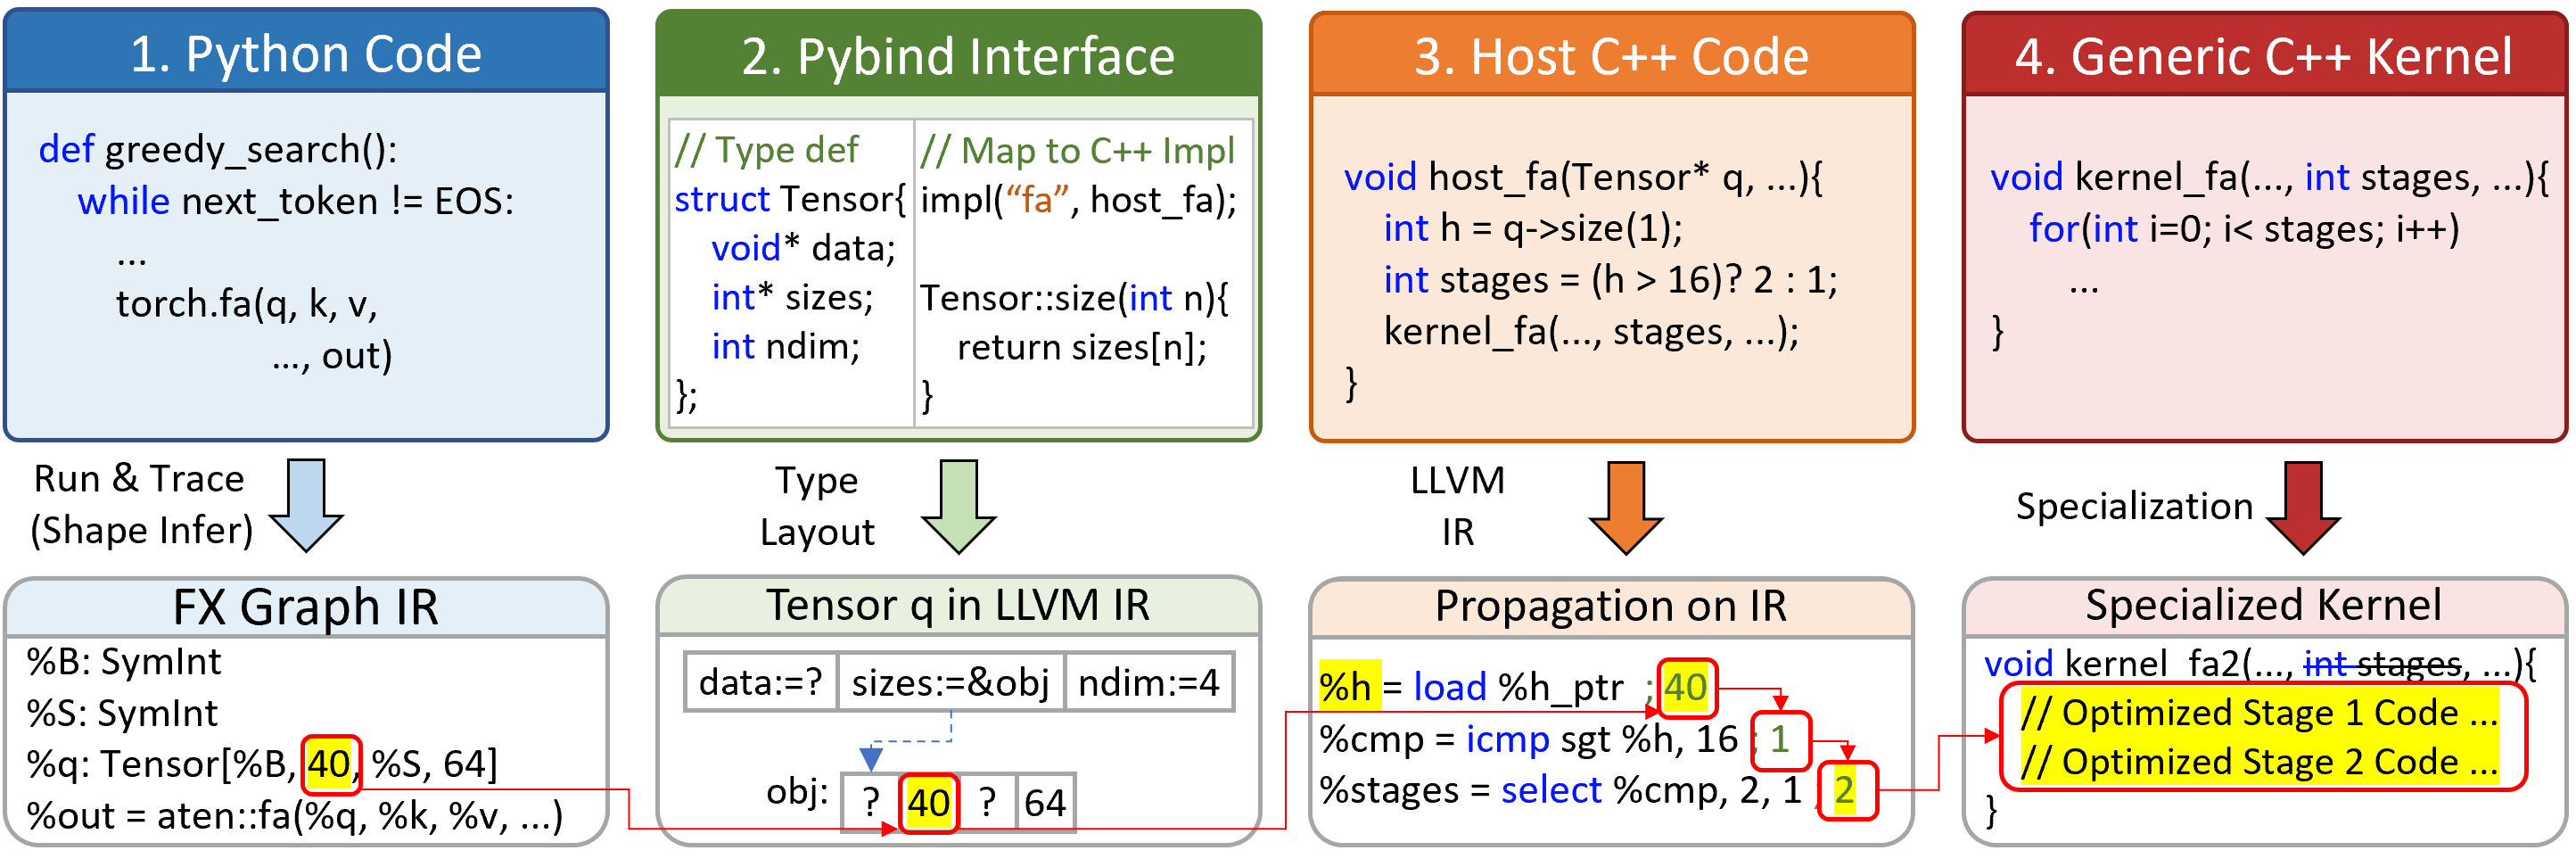
\includegraphics[width=\linewidth]{figures/motivation/motivating-example.png}
	\caption{A simplified Graph-to-C++ constant-propagation opportunity for Flash Attention. A model-fixed graph dimension (e.g., \texttt{q->size(1) = 40}) flows into C++ host code and determines the launch-site schedule parameter \texttt{stages = 2}, enabling specialization of \texttt{kernel\_fa} into \texttt{kernel\_fa2}.}
	\Description{Diagram showing a graph-level model constant materialized in the abstract C++ entry state and propagated through host code to a device-kernel launch site.}
	\label{fig:motivating-example}
\end{figure}

\subsubsection{\DIFdel{Disadvantages of Generic Kernels and Manually Specialized Libraries}\DIFadd{Limitations of the Two Expert-Written Operator-Library Designs}}
\label{sec:motivation:disadvantages}

\paragraph*{Bottleneck Analysis \DIFdel{for Generic Kernels}\DIFadd{of Schedule-Generic Implementations}.}

{\color{red}%
\DIFdel{%
Some operator libraries implement their kernels in the form of generic kernels, such as the built-in operator library of Ascend CANN. These kernels are not specialized mainly due to their complex schedule strategies and the great number of schedule parameters. In this design, almost all schedule parameters are passed as runtime arguments from the host. Since the compiler treats these parameters as variables, it cannot perform aggressive optimizations like constant folding. To understand the impact of this design, we examine the execution flow on Ascend, a DL accelerator based on SIMD execution model, as shown in }\autoref{fig:fa_on_ascend}\DIFdel{.
}
\par}
{\color{blue}%
Schedule-generic kernels support complex scheduling strategies by receiving numerous schedule parameters from the host at runtime. Because the compiler cannot treat these parameters as constants, optimizations such as constant folding and loop simplification remain limited. \autoref{fig:fa_on_ascend} illustrates the resulting overhead on Ascend.
\par}

{\color{red}%
\DIFdel{%
Ascend is a DL accelerator based on SIMD execution model, featuring diverse compute and storage units for handling different types of tensor computations and data movement operations. Specifically, the Cube and Vector units execute the primary tensor operations (e.g., MatMul on Cube and Softmax on Vector), while the architecture provides sophisticated programmable memory hierarchies. The kernel must explicitly manage the chunk size and data layout at every level, as well as the data movement and layout transformations between these levels. Besides, the Scalar unit acts as the central control unit, responsible for scalar data processing, instruction dispatch, and handling control flows (such data paths are indicated by red dashed lines; for simplicity, only some are shown). For example, the kernel moves a tile of the tensor $Q_{GM}$ from the global memory (GM) to the L1 memory unit at a time, denoted as $Q_{L1}$. During this data movement, the Scalar unit is responsible for calculating the starting memory address of tile $Q_{GM}$, implementing loop iterations, and loading or storing necessary scalar data (including schedule parameters and partial scalar intermediate results) from the global memory or the Unified Buffer (UB).
}
\par}
{\color{red}%
\DIFdel{%
In generic kernels, the Scalar unit may be over-occupied. Since the Scalar unit typically possesses much lower computing power than a general-purpose host CPU, excessive scalar calculations related to schedule parameters can overload the unit. Worse yet, excessive scalar intermediates may cause register spill, as there are only 32 general-purpose registers. As a result, the powerful Cube and Vector units will stall to await instruction dispatch or scalar operands. Furthermore, generic kernels often involve complex control flows (e.g., branching to handle different operator variants), which exerts heavy pressure on the instruction cache (I-Cache). Frequent instruction jumps in such complex logic inevitably lead to I-Cache misses and pipeline flushes. Finally, when loop bounds remain unknown at compile time, the compiler struggles to perform loop unrolling. Consequently, instruction scheduling is confined to the scope of a single iteration, preventing the effective overlapping of memory access and computation.
}
\par}
{\color{red}%
\DIFdel{%
We further study this impact by profiling key operators from the Qwen2.5-1.5B model on the Ascend NPU. }\autoref{fig:perf_stats}\DIFdel{ presents the Scalar unit occupancy (the proportion of active cycles during kernel execution) and I-Cache miss rates. The data reveals that the Scalar unit is active for 78\% to 91\% of total cycles, while I-Cache miss rates range from 3.1\% to 16.4\%.
}
\par}
{\color{blue}%
Ascend combines Cube and Vector compute units with a programmable memory hierarchy. Kernels explicitly manage tile sizes, data layouts, and data movement across memory levels, while the Scalar unit computes addresses and loop bounds, handles control flow, and dispatches instructions. For example, when moving a tile from $Q_{GM}$ in global memory (GM) to $Q_{L1}$ in L1 memory, the Scalar unit determines its starting address, advances the loop, and accesses schedule parameters and scalar intermediates in GM or the Unified Buffer (UB). The representative profiles in \autoref{fig:perf_stats} show high Scalar ratios and nonzero I-Cache miss rates for several of these kernels. These measurements motivate device-side specialization to reduce the scalar workload and improve instruction locality.
\par}

\begin{figure}[htbp]
	\centering
	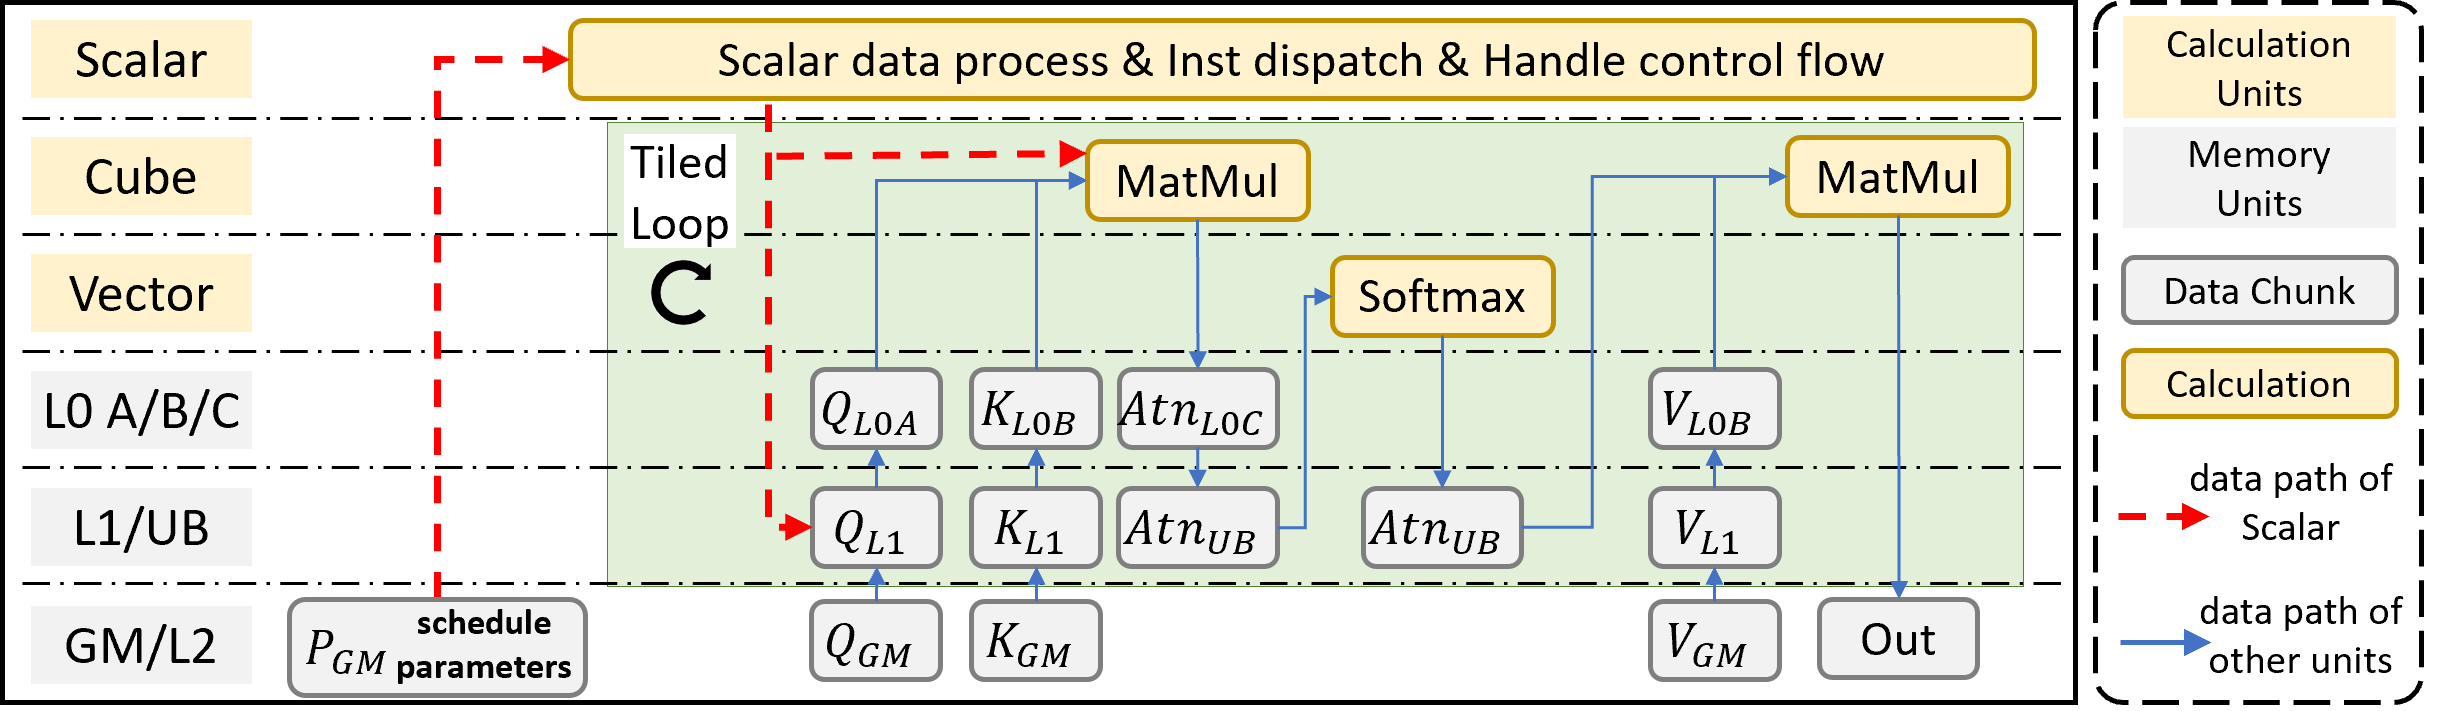
\includegraphics[width=0.8\textwidth]{figures/motivation/ascend-data-path.png}
	\caption{Execution flow of Flash Attention kernel \texttt{kernel\_fa} on the Ascend architecture.
		The \textbf{Scalar} unit acts as the central scheduler.
		It continuously performs scalar calculations and dispatches instructions based on runtime parameters.
		The heavy scalar workload required by generic kernels may lead to a scalar bottleneck.}
	\Description{Diagram showing the interaction between Scalar, Cube, Vector, L1, and GM units on Ascend.}
	\label{fig:fa_on_ascend}
\end{figure}

% Keep this paragraph in its original word-level LaTeXDiff form.
\paragraph*{Code Bloat in \DIFdel{Manually Specialized Libraries}\DIFadd{Schedule-Fixed Implementations}.}
High-performance GPU libraries \DIFdel{like }\DIFadd{such as }FlashInfer~\cite{ye2025flashinfer} rely on C++ template metaprogramming to enable aggressive compiler optimizations.
To avoid runtime JIT overhead, \DIFdel{these }\DIFadd{such }libraries pre-instantiate kernels for the Cartesian product of all template parameters.
As described in \autoref{eq:flash_attention}, FA's configuration space includes head dimensions ($d_k \in \{64, 128, 256\}$), mask types, GQA sizes, and position encodings.
Combined with \DIFdel{tile size}\DIFadd{tile-size} configurations, this results in over \DIFdel{1000}\DIFadd{1,000} binary instantiations, yet a specific model \DIFdel{like \textbf{Qwen2-1.5B} }\DIFdel{utilizes}\DIFadd{uses} only $\sim$10 kernels.
This pre-instantiation strategy, while manageable on GPUs, is ill-suited for Ascend due to its more complex schedule parameters, forcing \DIFdel{Ascend libraries }\DIFadd{their Ascend counterparts }to rely on \DIFdel{suboptimal generic kernels}\DIFadd{schedule-generic kernels with limited compile-time optimization}.

\begin{figure}[htbp]
	\centering
	\begin{minipage}{0.47\textwidth}
		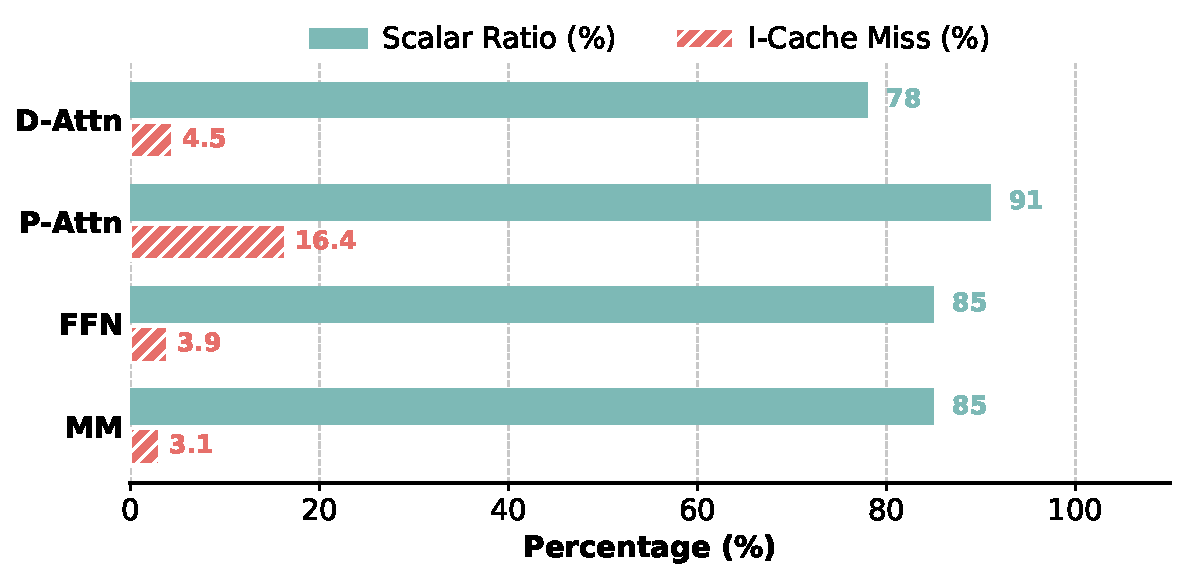
\includegraphics[width=\linewidth]{figures/motivation/metrics_analysis.pdf}
		\caption{Performance profiles of schedule-generic kernels, where lower values are better for both metrics: Decoding Attention (\textbf{D-Attn}), Prefill Attention (\textbf{P-Attn}), Feed Forward Networks (\textbf{FFN}), and MatMul (\textbf{MM}).}
		\Description{Bar chart showing scalar instruction ratio and I-Cache miss rate for different operators.}
		\label{fig:perf_stats}
	\end{minipage}
	\hfill
	\begin{minipage}{0.47\textwidth}
		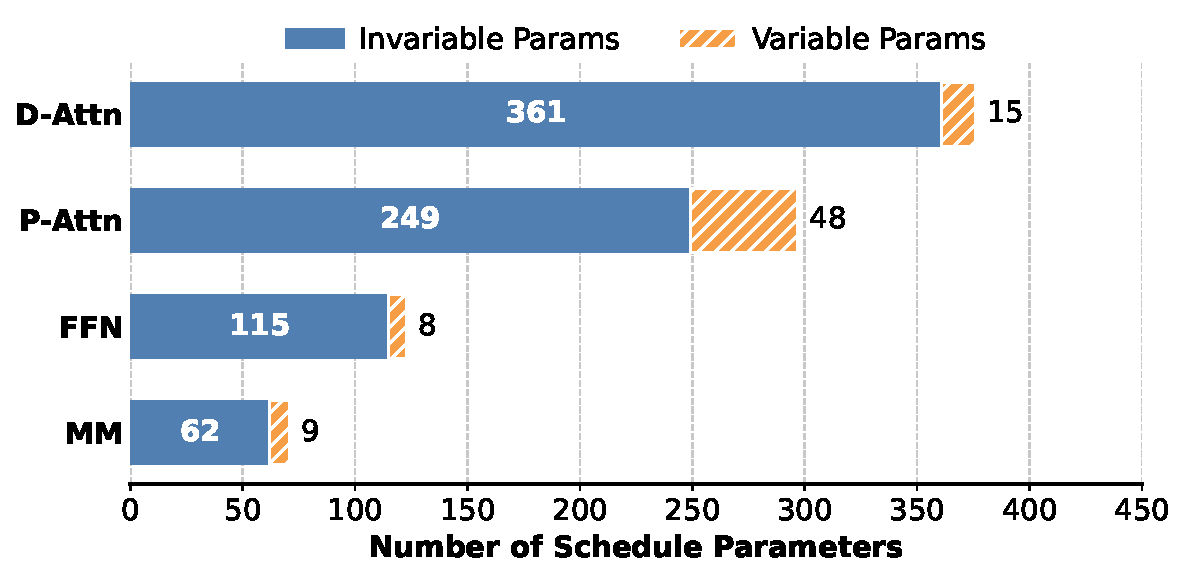
\includegraphics[width=\linewidth]{figures/motivation/parameter_breakdown.pdf}
		\caption{Number of schedule parameters of representative kernels. The vast majority are runtime invariants (Invariable Params), validating the potential for specialization.}
		\Description{Bar chart showing the breakdown of schedule parameters into variable and invariable categories.}
		\label{fig:param_stats}
	\end{minipage}
\end{figure}

% Keep this subsection in its original word-level LaTeXDiff form.
\subsubsection{Why Is Automatic \DIFdel{Kernel }\DIFadd{Model-Specific }Specialization Beneficial?}

We further analyze the schedule parameters of key operators from the \textbf{Qwen2.5-1.5B} model, classifying them into \textit{invariable parameters} (constants derived from model configuration) and \textit{variable parameters} (runtime-dependent values such as batch size and sequence length).
\autoref{fig:param_stats} reveals that the overwhelming majority of kernel parameters are invariable.
Propagating model-specific constants to resolve schedule parameters at compile time yields two benefits: (1) for \DIFdel{generic kernels}\DIFadd{schedule-generic implementations}, it enables model-specific \DIFadd{kernel }specialization with aggressive constant folding, reducing scalar overhead and I-Cache misses; (2) for \DIFdel{manually specialized libraries}\DIFadd{schedule-fixed implementations}, it makes kernel dispatch paths deterministic, enabling precise pruning of unused binaries.

\DIFadd{In addition, the sensitivity study in \S\ref{sec:eval:sensitivity} analyzes which schedule parameters have the greatest effect on performance. It shows that a small subset of parameters on the kernel's hot path accounts for most of the performance gain.}\par

\subsection{Challenges and Design Insights}
\label{sec:motivation:challenges}

{\color{red}%
\DIFdel{%
Achieving automatic kernel specialization requires analyzing the value flow from Python down to C++, which presents two major challenges that cannot be properly addressed by existing static analysis.
}
\par}
{\color{blue}%
Achieving automatic model-specific specialization requires transferring graph-level facts into C++ compilation and preserving them through host-side control flow. These steps present two challenges not directly addressed by existing static analyses.
\par}

\subsubsection{Challenge 1: \DIFdel{The cross-language semantic gap}\DIFadd{Reconstructing Cross-Language Calling Contexts}.}

{\color{red}%
\DIFdel{%
Achieving automatic kernel specialization requires reconstructing the calling context for C++ operator functions, i.e., determining the tensor shapes and operator attribute values. As shown in }\autoref{fig:motivating-example}\DIFdel{, these values are instantiated on the Python side and passed through the FFI layer to C++. However, reconstructing this cross-language value flow faces significant challenges.
}
\par}
{\color{blue}%
The first challenge is the Python/C++ semantic gap: Graph IR constants and symbolic dimensions must be mapped to the memory states of their underlying C++ objects before LLVM can use them as compile-time facts. This mapping is not a direct binding between the arguments of a Graph IR node and C++ parameters. Graph IR records typed values and shapes, whereas composite C++ parameters such as \texttt{Tensor}, \texttt{List}, and \texttt{Optional} use nested object layouts; after lowering, an access such as \texttt{query->size(1)} becomes pointer arithmetic and \texttt{load} instructions. The analyzer must therefore reconstruct the corresponding base objects, pointers, field offsets, and field values, preserving concrete dimensions as constants and symbolic dimensions as unknown.
\par}

{\color{red}%
\DIFdel{%
Existing cross-language analysis methods~}\mbox{\cite{kan2024taint4javac,Monat2021PythonC}}\hspace{0pt}\DIFdel{ typically employ abstract interpretation at the FFI API level, modeling each cross-language call as state transitions in an abstract domain. While general-purpose, this approach is ill-suited for DL systems for two reasons. First, the FFI layer contains substantial glue code for type conversions, dynamic dispatch, and reference counting, operations that are essential for language interoperability but irrelevant to the constant values we aim to extract. Analyzing this glue code is both computationally expensive and unnecessary for our goal. Second, the Python-side Graph Executor, which orchestrates operator invocations based on Graph IR, comprises complex logic spanning thousands of lines of code. Performing full abstract interpretation over this codebase is prohibitively expensive. These factors render traditional approaches impractical for reconstructing operator calling contexts in DL systems.
}
\par}
{\color{blue}%
Existing cross-language analyses broadly follow two approaches: multilanguage abstract interpretation jointly analyzes programs on both sides of an FFI boundary~\cite{Monat2021PythonC}, while specification-based methods summarize native behavior under a cross-language caller context~\cite{kan2024taint4javac}. The former would have to traverse the Python Graph Executor and FFI glue for dispatch, type conversion, object construction, and reference counting, which is expensive and largely irrelevant to graph-level constants. The latter assumes or derives a cross-language caller context but does not define how Graph IR metadata should materialize the field-sensitive C++ entry state required by LLVM.
\par}

{\color{red}%
\DIFdel{%
Insight: Semantic modeling of core data types in DL systems. Instead of analyzing FFI glue code and Python source code, we propose a cross-language semantic modeling approach grounded in two observations: (1) Finite and Stable Core Types: Data types used for cross-language interaction in DL systems are highly convergent and stable (Tensor, Array, etc.), enabling comprehensive and precise semantic modeling. (2) Extract Constant Information from Graph IR: DL systems compile models and represent them using Graph IR (e.g., ATen IR), which contains precise information regarding operator input parameters, enabling direct extraction of semantic values without analyzing Python source code. Specifically, model-specific constants are captured as exact values from tracing, while dynamic dimensions are represented as symbolic variables. Building on these insights, we directly map computation graph node information to the abstract states of C++ entry functions, achieving high-precision reconstruction of C++ contexts while avoiding the overhead of analyzing complex FFI glue code.
}
\par}
{\color{blue}%
\textit{Insight: Type-directed calling-context construction.} DL operator interfaces use a limited set of parameter types, and their C++ interface layouts are stable within a backend. We can therefore define a context-update rule for each type and use Graph IR shapes and attributes to construct an accurate C++ operator calling context directly. This approach avoids analyzing FFI glue code; \autoref{tab:semantic-rules} formalizes the context-update rules used by TilingInfer.
\par}

\begin{figure}[htbp]
	\centering
	\begin{minipage}{0.39\textwidth}
		\begin{lstlisting}[
    language=C++,
    frame=single,
    caption={Early-exit path example.},
    basicstyle=\ttfamily\footnotesize,
    columns=fullflexible,
    framesep=1.5pt,
    aboveskip=0pt,
    belowskip=0pt,
    label={lst:early_return_code}
  ]
const status SUCCESS=0, ERROR=-1;
status check(int s1, int s2) {
  if(s1 != s2) return ERROR;
  return SUCCESS;
}
status set_t(int sk, int sv, int* t) {
  int e = check(sk, sv);
  if(e != SUCCESS) {
    print("error"); return e;
  }
  *t=32; // Tiling
  return SUCCESS;
}
  \end{lstlisting}
	\end{minipage}
	\hspace{0.04\textwidth}
	\begin{minipage}{0.47\textwidth}
		\centering
		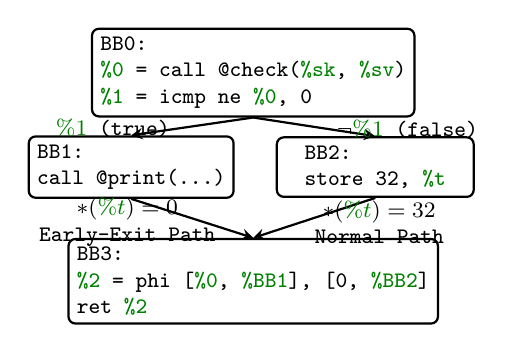
\begin{tikzpicture}[
					bb/.style={
							rectangle,
							rounded corners=2.5pt,
							draw=black,
							thick,
							minimum width=2.5cm,
							inner sep=3pt,
							font=\ttfamily\footnotesize,
							align=left
						},
					edge_label/.style={
							font=\ttfamily\footnotesize,
							midway
						},
					>=stealth
				]
				\node[bb] (BB0) at (0, 0) {
				\textbf{BB0:}\\
				{\color{green!50!black}\%0} = call @check({\color{green!50!black}\%sk}, {\color{green!50!black}\%sv})\\
				{\color{green!50!black}\%1} = icmp ne {\color{green!50!black}\%0}, 0
				};

				\node[bb] (BB1) at (-1.55, -1.2) {
					\textbf{BB1:}\\
					call @print(...)
				};

				\node[bb] (BB2) at (1.55, -1.2) {
					\textbf{BB2:}\\
					store 32, {\color{green!50!black}\%t}
				};

				\node[bb] (BB3) at (0, -2.65) {
					\textbf{BB3:}\\
					{\color{green!50!black}\%2} = phi [{\color{green!50!black}\%0}, {\color{green!50!black}\%BB1}], [0, {\color{green!50!black}\%BB2}]\\
					ret {\color{green!50!black}\%2}
				};

				\draw[->, thick] (BB0.south) -- (BB1.north)
				node[edge_label, left, pos=0.6] {{\color{green!50!black}$\%1$} (true)};
				\draw[->, thick] (BB0.south) -- (BB2.north)
				node[edge_label, right, pos=0.6] {$\neg${\color{green!50!black}$\%1$} (false)};
				\draw[->, thick] (BB1.south) -- (BB3.north);
				\draw[->, thick] (BB2.south) -- (BB3.north);

				\node[font=\ttfamily\footnotesize, align=center] at (-1.6, -1.9) {
				$*({\color{green!50!black}\%t}) = 0$\\
				{Early-Exit Path}
				};
				\node[font=\ttfamily\footnotesize, align=center] at (1.6, -1.9) {
				$*({\color{green!50!black}\%t}) = 32$\\
				{Normal Path}
				};
		\end{tikzpicture}
		\caption{Control Flow Graph (CFG) of \texttt{set\_t}'s LLVM IR. Each node is a basic block containing LLVM IR instructions. Edges are labeled with branch conditions.}
		\label{fig:set_t_cfg}
	\end{minipage}
	\Description{Control flow graph showing an early-exit path in LLVM IR.}
\end{figure}

\color{black}
\subsubsection{Challenge 2: Shape Checkers Leading to Early-Exit Paths}
\leavevmode

{\color{red}%
\DIFdel{%
Operator libraries enforce shape constraints through runtime shape checkers to ensure memory safety and computational correctness. As defined in }\autoref{eq:flash_attention}\DIFdel{, the Flash Attention operator imposes one constraint that the sequence lengths of $K$ and $V$ must be equal ($S_k = S_v$). Violations of these constraints trigger early exits with error codes.
}
\par}
{\color{blue}%
The second challenge is preserving constant-propagation precision across shape-checker-induced early-exit paths without expensive path-sensitive analysis. Operator libraries enforce constraints for memory safety and correctness; for example, Flash Attention requires equal key and value sequence lengths ($S_k=S_v$). Because these dimensions may remain symbolic, the compiler cannot decide whether a check succeeds. An early-exit path then bypasses assignments performed on the normal path, and merging the two states can obscure constants.
\par}

{\color{red}%
\DIFdel{%
}\autoref{lst:early_return_code}\DIFdel{ illustrates this pattern with a simplified example. The function check verifies whether two sequence lengths (denoted as s1 and s2) match, returning SUCCESS (0) if they are equal or ERROR (-1) otherwise. The function set\_t uses this checker to validate the sequence lengths before computing the tiling parameter t=32. Since these dimensions are dynamic at compile time, the compiler cannot determine whether the check will succeed or fail.
}
\par}
{\color{red}%
\DIFdel{%
}\autoref{fig:set_t_cfg}\DIFdel{ shows the corresponding CFG. The entry block BB0 calls @check and branches based on the result: the true branch leads to BB1 (error path), while the false branch leads to BB2 (normal path) where t=32 is defined. Both paths converge at BB3. At this merging site, standard path-insensitive analysis cannot determine whether the definition of t originates from BB2 or is undefined from BB1, resulting in a polluted abstract state $\{t \in \{0, 32\}\}$ that prevents constant propagation.
}
\par}
{\color{blue}%
In \autoref{lst:early_return_code}, \texttt{check} returns \texttt{SUCCESS} or \texttt{ERROR}, and \texttt{set\_t} computes \texttt{t=32} only after the check succeeds. The CFG in \autoref{fig:set_t_cfg} branches at \textbf{BB0}: \textbf{BB1} returns through the early-exit path without defining \texttt{t}, whereas \textbf{BB2} defines it before both paths reach \textbf{BB3}. If \texttt{t} initially holds 0, path-insensitive merging yields $\{0,32\}$ rather than the normal-path constant 32. Enumerating all paths would avoid this pollution, but nested shape checkers make full path-sensitive analysis impractical.
\par}

{\color{red}%
\DIFdel{%
Insight: Conditional Return-Value Flow. The key to identifying early-exit paths lies in analyzing the relationship between path guards and the semantic meaning of return values. Since shape checkers assign different constant values to the return variable on different execution paths (e.g., SUCCESS on the normal path and ERROR on the error path), we can determine whether a path is an early-exit by examining whether the path guard implies an error return value. Specifically, we maintain path-sensitive guards and propagate them through the control flow. If a path guard implies that the return value equals an error code, the path is identified as an early-exit path; otherwise, it is conservatively treated as a normal path. During constant propagation, value states from confirmed early-exit paths are prevented from propagating to merge points, thereby avoiding state pollution. In }\autoref{fig:set_t_cfg}\DIFdel{, the branch condition at BB0 is $\%1 = (\%0 \neq 0)$, where $\%0$ is the return value of @check. When the guard $\%1 = true$ holds, we have $\%0 \neq 0$, which implies $\%0 \neq SUCCESS$; hence the return value represents an error, and the path $BB0 \rightarrow BB1 \rightarrow BB3$ guarded by $\%1$ is an early-exit path. Conversely, when the guard $\neg\%1$ holds, we have $\%0 = 0 = SUCCESS$; hence the return value represents success, and the path $BB0 \rightarrow BB2 \rightarrow BB3$ guarded by $\neg\%1$ is a normal path.
}
\par}
{\color{blue}%
\textit{Insight: Conditional Return-Value Flow.} CRVFG-based normal-path reasoning traces only the conditional flow of status return values and compares them with configured success and error sets. In the example, the guard $\%1=(\%0\neq0)$ being true implies that \texttt{check}'s return value is not \texttt{SUCCESS}, so \textbf{BB0}$\rightarrow$\textbf{BB1} is an early-exit edge; its false branch is the normal edge. Confirmed early-exit-edge states are excluded from normal-path merges, while unclassified edges are retained conservatively.
\par}
